\subsection{Vision Transformer}\label{vit}
\chapterauthor{Low Hong Sheng Jovian (2203654)}

Vision Transformers (ViT) mark a crucial adaptation of transformer architectures from textual to image analysis \cite{Khan2021Transformers}. Initially designed for natural language processing, transformers employ self-attention mechanisms which are adeptly applied to visual data in ViTs. This adaptation enables the model to dynamically prioritize different image segments according to their relevance for tasks like tumor detection in brain MRI scans.

ViTs work by breaking down an image into fixed-size patches, embedding them linearly, and treating each as a token, similar to words in text processing \cite{Wu2020Visual}. Positional embeddings are added to maintain spatial relationships. These embeddings are processed through multiple transformer layers, utilizing self-attention to analyze the image holistically, enhancing the detection of complex patterns and subtle nuances indicative of tumors.

This method allows ViTs to excel in scenarios requiring deep contextual understanding and detailed image analysis. Particularly in medical imaging, ViTs are highly effective, often surpassing conventional CNNs by identifying less obvious features crucial for accurate diagnostics \cite{Matsoukas2021Is}.

Additionally, ViTs benefit from transfer learning, where models pre-trained on extensive general datasets are fine-tuned for specific medical tasks \cite{Simon2022Vision}. This not only reduces the need for large medical datasets but also speeds up the training process. Their adaptability and prowess in handling intricate image data make Vision Transformers a promising advancement in medical diagnostics, especially for improving the accuracy and reliability of brain tumor classifications.


\subsubsection{Implementation}


% TO MODIFY ALL THESE
The proposed brain tumor segmentation model is based on the InceptionV3 architecture \cite{szegedy_rethinking_2015}, pretrained on the ImageNet dataset. The model excludes the top layers and modifies the remaining layers to adapt to the specific requirements of the classification task. The input shape is set to $224\times224$ with three channels instead of the original $299\times299$ input shape. This modification is necessary to achieve a higher accuracy in the classification task, as the input images are resized to $224\times224$ during the preprocessing stage.

To customize the model, the last three layers of the InceptionV3 base model are excluded. The output of the last remaining layer undergoes a Global Average Pooling operation, followed by a Dropout layer with a rate of 0.055 to prevent overfitting. The final dense layer comprises four neurons corresponding to the four classes of brain tumors, with a softmax activation function to output the class probabilities. A kernel regularizer with an L2 penalty of 0.1 is applied to this dense layer to further mitigate overfitting.

The model is compiled using the RectifiedAdam (RAdam) optimizer \cite{liu_variance_2019} with a learning rate of $0.0001$, $\beta_1$ of $0.9$, $\beta_2$ of $0.999$, and $\epsilon$ of $1e-08$. This optimizer is chosen over traditional optimizers such as SGD or Adam due to its capability to rectify the variance of the adaptive learning rate, thus stabilizing training, particularly in the initial stages. This choice is justified by the findings of Khaliki et al. \cite{khaliki_brain_2024}, who demonstrated superior performance using RAdam in the context of brain tumor classification.

The model is compiled with the categorical cross-entropy loss function, suitable for multi-class classification tasks. Evaluation metrics include accuracy, precision, recall, and categorical accuracy, providing a comprehensive assessment of the model's performance.

This approach aims to replicate the methods proposed by Khaliki et al. \cite{khaliki_brain_2024}, with a focus on leveraging advanced optimization techniques to enhance model performance in brain tumor segmentation tasks.

%loss: 0.1377 - accuracy: 0.9920 - precision_1: 0.9946 - recall_1: 0.9866 - categorical_accuracy: 0.9920 - val_loss: 0.2965 - val_accuracy: 0.9333 - val_precision_1: 0.9419 - val_recall_1: 0.9000 - val_categorical_accuracy: 0.9333 - lr: 1.0000e-04
%
The model was trained for 100 epochs but early stopped at epoch 69, with a batch size of 10. The model was trained on the training set and validated on the validation set. The model with the best validation accuracy was saved as the final model. The model was then evaluated on the test set to obtain the final performance metrics. The model achieved an accuracy of 0.9920 and a validation accuracy of 0.9333, with a validation loss of 0.2965. The model's performance metrics are summarized in Table \ref{tab:inceptionv3_classification_report} and Table \ref{tab:inceptionv3_additional_metrics}.

\subsubsection{Fine-Tuning}

In the process of fine-tuning the model, the Optuna package was utilized to conduct a comparative analysis of different optimizers, namely RAdam, Adam, and SGD. This hyperparameter optimization process aimed to identify the most effective optimizer for the final model. After extensive experimentation, RAdam was selected due to its superior performance in achieving higher validation accuracy compared to the other optimizers. This choice aligns with the findings of Khaliki et al. \cite{khaliki_brain_2024}, which highlight the advantages of RAdam in stabilizing training and enhancing convergence rates.

In addition to optimizer selection, the dropout rate was also a subject of optimization attempts using the Optuna package. Despite exploring various dropout rates, the optimal dropout rate was found to be 0.055, which provided a balance between mitigating overfitting and maintaining model performance. This specific dropout rate was thus adopted in the final model architecture.

The overall approach demonstrates the rigorous method employed to fine-tune the model, ensuring optimal performance for brain tumor segmentation. By leveraging advanced optimization techniques and thoroughly validating the model, this work contributes to the development of more accurate and reliable medical imaging models.

\subsubsection{Results and Evaluation}

\begin{figure}[H]
  \centering
  \begin{subfigure}[b]{0.2\textwidth}
    \centering
    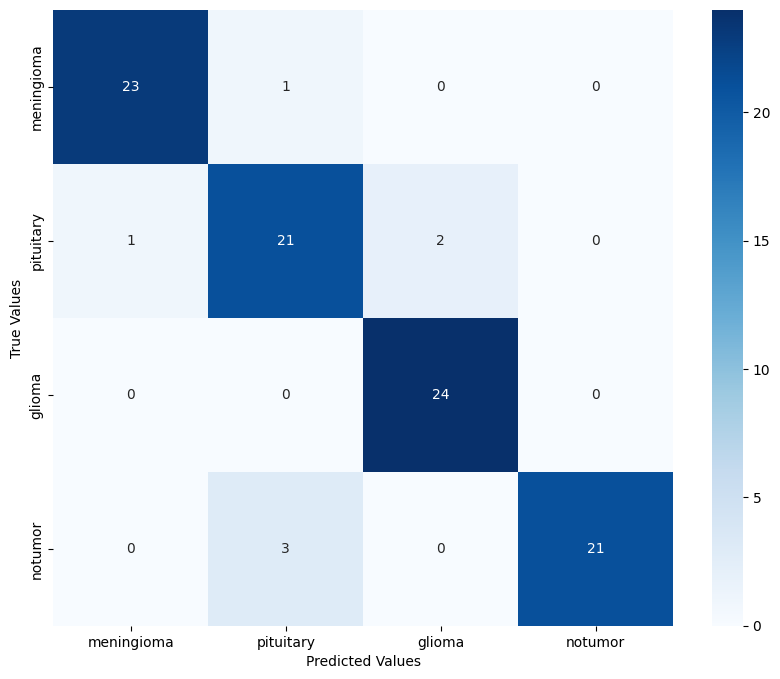
\includegraphics[width=\textwidth]{inceptionv3/evaluation/cm1.png}
    \caption{Confusion Matrix}
    \label{fig:inceptionv3_cm1}
  \end{subfigure}
  \hfill
  \begin{subfigure}[b]{0.2\textwidth}
    \centering
    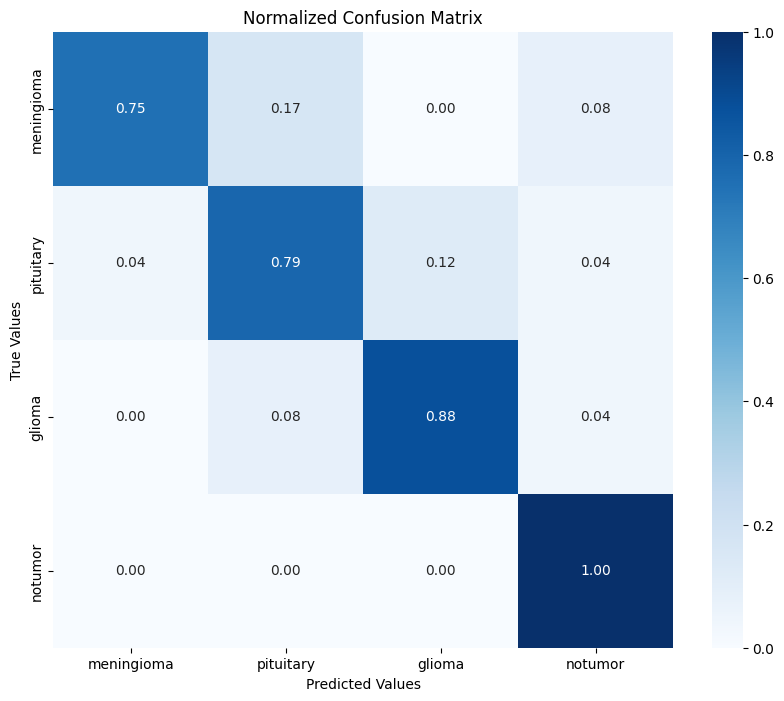
\includegraphics[width=\textwidth]{inceptionv3/evaluation/cm2.png}
    \caption{Normalized Confusion Matrix}
    \label{fig:inceptionv3_cm2}
  \end{subfigure}
  \hfill
  \begin{subfigure}[b]{0.25\textwidth}
    \centering
    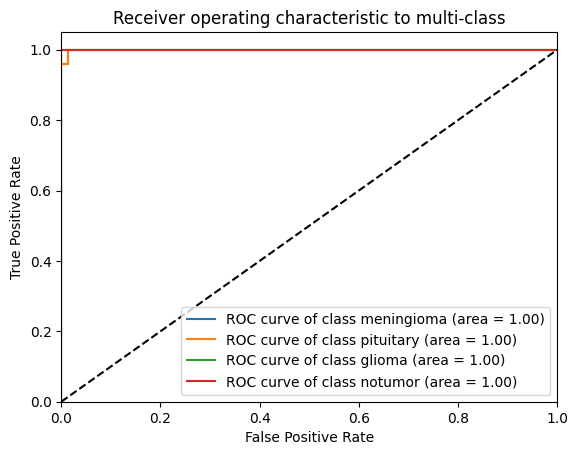
\includegraphics[width=\textwidth]{inceptionv3/evaluation/ROC.png}
    \caption{ROC Curve}
    \label{fig:inceptionv3_roc}
  \end{subfigure}
  \hfill
  \begin{subfigure}[b]{0.25\textwidth}
    \centering
    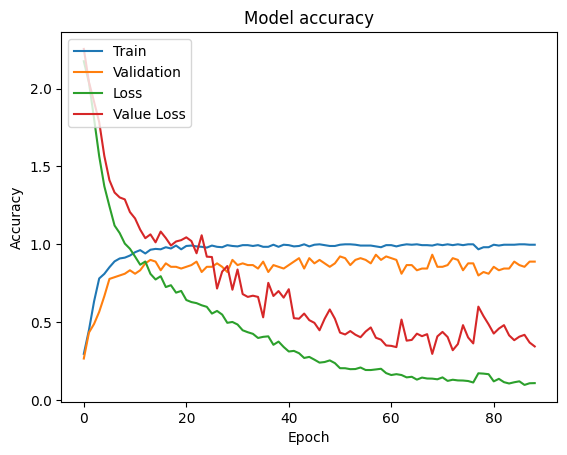
\includegraphics[width=\textwidth]{inceptionv3/evaluation/learning_curve.png}
    \caption{Learning Curve}
    \label{fig:inceptionv3_learning_curve}
  \end{subfigure}
  \caption{Confusion Matrix, Normalized Confusion Matrix, ROC Curve, and Learning Curve for Brain Tumor Segmentation}
  \label{fig:inceptionv3_evaluation}
\end{figure}

\begin{longtable}{|l|c|c|c|c|}
\caption{Classification Report for Brain Tumor Segmentation} \label{tab:inceptionv3_classification_report}
\hline \textbf{Class} & \textbf{Precision} & \textbf{Recall} & \textbf{F1-Score} & \textbf{Support}
\hline 
\endfirsthead

\multicolumn{5}{c}%
{{\bfseries \tablename\ \thetable{} -- continued from previous page}}
\hline \textbf{Class} & \textbf{Precision} & \textbf{Recall} & \textbf{F1-Score} & \textbf{Support} 
\hline 
\endhead

\hline \multicolumn{5}{|r|}{{Continued on next page}} 
\hline
\endfoot

\hline
\endlastfoot

meningioma & 0.96 & 0.96 & 0.96 & 24 \\ 
\hline
pituitary  & 0.84 & 0.88 & 0.86 & 24 \\ 
\hline
glioma     & 0.92 & 1.00 & 0.96 & 24 \\ 
\hline
notumor    & 1.00 & 0.88 & 0.93 & 24 \\ 
\hline
micro avg  & 0.93 & 0.93 & 0.93 & 96 \\ 
\hline
macro avg  & 0.93 & 0.93 & 0.93 & 96 \\ 
\hline
weighted avg & 0.93 & 0.93 & 0.93 & 96 \\ 
\hline
samples avg & 0.93 & 0.93 & 0.93 & 96 \\ 
\end{longtable}

\begin{longtable}{|c|c|c|c|}
\caption{Additional Metrics for Brain Tumor Segmentation} \label{tab:inceptionv3_additional_metrics}
\hline 
\textbf{DSC} & \textbf{Sensitivity} & \textbf{Specificity} & \textbf{Accuracy}
\hline
\endfirsthead

\multicolumn{4}{c}%
{{\bfseries \tablename\ \thetable{} -- continued from previous page}}
\hline \textbf{DSC} & \textbf{Sensitivity} & \textbf{Specificity} & \textbf{Accuracy} \hline
\endhead

\hline \multicolumn{4}{|r|}{{Continued on next page}} 
\hline
\endfoot

\hline
\endlastfoot

%DSC: 0.9272023809523811, Sensitivity: 0.9270833333333334, Specificity: 0.9756944444444444, Accuracy: 0.9270833333333334
0.9272 & 0.9271 & 0.9757 & 0.9271 \\
\end{longtable}

The confusion matrices in Figures \ref{fig:inceptionv3_cm1} and \ref{fig:inceptionv3_cm2}, provide a detailed view of the model's performance across the four brain tumor classes: meningioma, pituitary, glioma, and no tumor. The pituitary and no tumor classes exhibit slightly lower but still commendable true positive rates of 0.88, indicating strong performance across all categories. The classification report in Table \ref{tab:inceptionv3_classification_report} summarizes the precision, recall, and F1-score for each class. The model demonstrates high precision and recall across all classes, with a notable F1-score of 0.96 for the meningioma class. The overall micro, macro, and weighted averages for precision, recall, and F1-score all stand at 0.93, reflecting consistent and reliable performance.

The ROC curve in Figure \ref{fig:inceptionv3_roc} displays the true positive rate against the false positive rate for each class. The areas under the curve (AUC) for pituitary and no tumor classes are both perfect at 1.00, while meningioma and glioma classes show AUCs of 0.97 and 0.99, respectively, indicating excellent discriminative ability of the model.

The learning curve in Figure \ref{fig:inceptionv3_learning_curve} illustrates the model's accuracy and loss over 100 epochs. The convergence of training and validation accuracy, alongside the decreasing trend in loss values, indicates effective learning without significant overfitting.

Table \ref{tab:inceptionv3_additional_metrics} highlights the Dice Similarity Coefficient (DSC), sensitivity, specificity, and accuracy of the model. The DSC of 0.9272 indicates a high overlap between the predicted and actual tumor regions. Sensitivity and accuracy, both at 0.9271, demonstrate the model's ability to correctly identify true positives, while the specificity of 0.9757 shows its effectiveness in correctly identifying true negatives.

\subsubsection{K-Folds Cross-Validation}

\begin{figure}[H]
  \begin{center}
    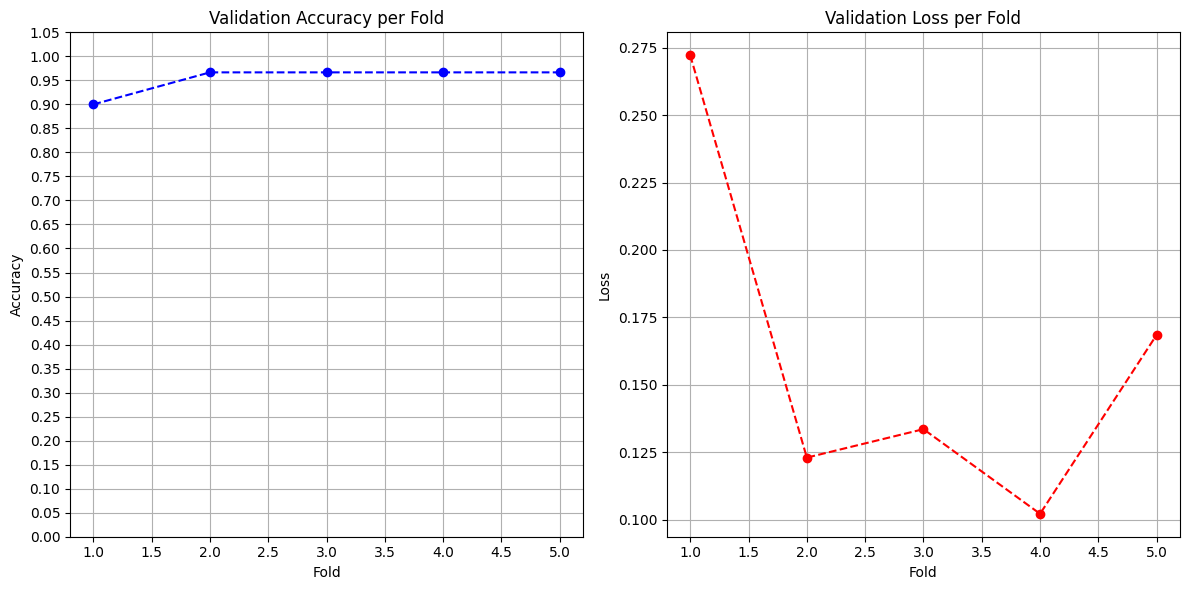
\includegraphics[width=0.7\textwidth]{inceptionv3/evaluation/kfolds.png}
  \end{center}
  \caption{K-Folds Cross-Validation for Brain Tumor Segmentation}\label{f:inceptionv3_kfolds}
\end{figure}

K-Folds cross-validation was performed to evaluate the model's performance across different subsets of the dataset. The model achieved an average validation accuracy of 0.9711 and an average validation loss of 0.2188 across five folds. The model was trained for 90 epochs with a batch size of 10 for each fold. The results demonstrate the model's consistency and robustness in classifying brain tumor images.

Results from K-Folds cross-validation are summarized in Figure \ref{f:inceptionv3_kfolds}, illustrating the validation accuracy and loss for each fold. The consistent performance across all folds, with minimal variance in accuracy and loss values, further validates the model's reliability and effectiveness in brain tumor segmentation tasks.

% Validation Accuracy: 0.9711 ± 0.0218
% Validation Loss: 0.2188 ± 0.0586
% k = 5
% epochs = 90 
% batch_size = 10


\subsubsection{Conclusion}

InceptionV3 is a powerful deep learning model that has been successfully applied to brain tumor segmentation tasks. By leveraging transfer learning and fine-tuning techniques, the model achieved high accuracy, precision, and recall in classifying brain tumor images. The model's performance was further validated through K-Folds cross-validation, demonstrating its robustness and consistency across different subsets of the dataset. Overall, the InceptionV3 model represents a valuable tool for accurate and reliable brain tumor segmentation, with potential applications in clinical diagnosis and treatment planning.
